% 第三章 基于YOLO的目标检测

\chapter{基于YOLO的目标检测}

\section{卷积神经网络介绍}
卷积神经网络(convolutional neural network, CNN)\cite{lecun1989}是一种专门用来处理具有类似网格结构的数据(如图像)的神经网络\cite{Goodfellow-et-al-2016}。其模拟了生物视觉神经的结构,对传统的神经网络做了一定的改变:将相邻两层神经元之间的全连接改为局部连接,并且同一层内的神经元共享权值。这些改变大大减少了神经网络的参数数量,降低了模型的复杂度,使得网络变得更容易训练。这种网络结构能够直接使用图像作为网络输入,避免了传统算法中人工提取特征的过程,在目标识别、图像分割、目标分类等很多任务中表现突出,得到了学术界与工业界的广泛关注和研究,已被大量应用于计算机视觉的各个领域中。


%\subsection{人工神经网络}
%\subsection{深度学习}
%\subsection{卷积神经网络的历史}

%------------------------------------------------------------------------------------
\subsection{卷积运算及其基本思想}
\subsubsection{卷积运算}
% ref: 吴文正,ch2.3.1,p18
数学上卷积运算包括连续卷积运算和离散卷积运算,它们的定义分别为:
%
\begin{equation}\label{eq:3_1_0}
y(t) = (x*w)(t) = \int_{-\infty}^{\infty}x(a)w(t-a)da
\end{equation}
\begin{equation}
y(n) = (x*w)(n) = \sum_{-\infty}^{\infty}x(i)h(n-i)
\end{equation}
其中的参数$x$是输入,参数$w$被称为核函数(kernel function)。星号表示卷积运算。注意到公式中将核函数进行了翻转,即当输入x的索引增大时,核w的索引是在减小的。通过翻转,卷积获得了可交换的性质,即$x*w=w*x$。

卷积神经网络中的卷积操作是对二维数组进行的,因此是二维离散卷积。而与常规的卷积不同的是,卷积神经网络的卷积计算中并没有进行翻转:
%
\begin{equation}
S(i,j) = (I*K)(i,j) = \sum\limits_{m} \sum\limits_{n} I(i+m,j+n)K(m,n)
\end{equation}
这种计算也被称为互相关函数(cross correlation),卷积核也被称为滤波器(filter)。

%------------------------------------------------------------------------------------
\subsubsection{卷积运算的基本思想}
% DL book, ch9.2, p313.
% 何鹏举,ch2.2,p16; 黄咨,ch3.3,p48.
% http://blog.csdn.net/zlrai5895/article/details/78634800?locationNum=6&fps=1
神经网络在过去几十年经历了多次起起落落,是因为其应用存在着很多困难。当网络较浅时,其无法刻画复杂的非线性关系,因此对于较多的数据和复杂的模式,无法得到理想的分类或预测性能;而如果网络很深或求解问题规模较大,则网络内的参数数量会急剧增加,运算量也会成指数级增长,导致训练无法完成。
卷积神经网络将卷积运算引入神经网络,而卷积运算包含了三个改进神经网络算法的重要思想:稀疏连接、参数共享和等变表示。

(1) 稀疏连接(局部感知)

传统神经网络使用矩阵乘法来建立各层网络的输入与输出之间的关系。参数矩阵中的每个元素都描述了上一层网络中某个神经元的输出与下一层网络的某个神经元的输入之间的交互,即每个输出单元与每个输入单元都存在着联系。然而,卷积网络具有稀疏连接的特点。输入图像中可能包含几万甚至几百万的像素点,但并没有必要让每个神经元都对整幅图像进行感知,因为局部区域内的像素联系比较大,而距离远的像素之间通常并没有很强的相关性。
使用只包含几十到几百个像素的小尺寸的卷积核,就可以检测图像中局部的特征,如边缘等。稀疏连接可以大大减少模型中的参数数量。

局部连接虽然使得每个神经元只与其前一层中很少的神经元有联系,但由于卷积神经网络有多层,通过层层的传递,处于网络中更深层的神经元实际上与相当多的浅层神经元之间存在着联系,它们比处在浅层的神经元具有更大的接受域。也就是说,深层的神经元将浅层神经元中的局部信息逐渐综合起来,从而得到了全局信息。这种模式非常类似于人类由局部到全局的视觉感知过程,因此稀疏连接的特性也被称为局部感知。

\begin{figure}[htb] %稀疏连接与全连接的对比;更深层的神经元具有更大的接受域
	\centering
	\begin{minipage}[c]{0.48\textwidth}
		\centering
		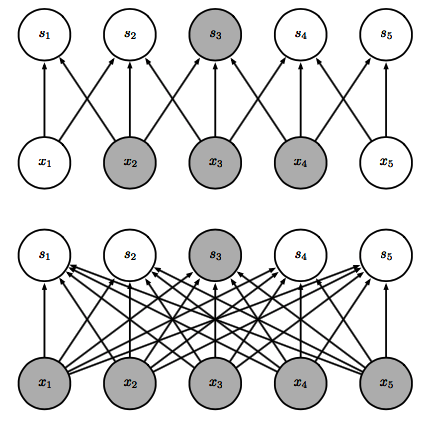
\includegraphics[width=3in]{figures/3_1_稀疏连接与全连接的对比}
		\caption{稀疏连接与全连接的对比}
	\end{minipage}
	\hfill
	\begin{minipage}[c]{0.48\textwidth}
		\centering
		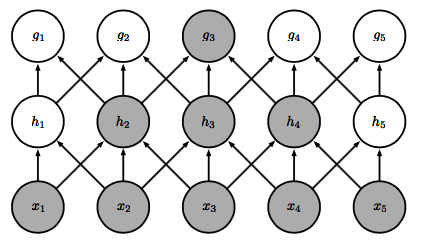
\includegraphics[width=3in]{figures/3_1_更深层的神经元具有更大的接受域}
		\caption{更深层的神经元具有更大的接受域}
	\end{minipage}
\end{figure}

(2)参数共享

参数共享是指对于不同的神经元使用相同的权重参数。在传统神经网络中,每层网络的权重矩阵W中的元素都仅仅被使用了一次,这是非常低效的。而在卷积神经网络中,卷积层通过平移卷积核遍历了整个特征平面,也就是说每个卷积核内的参数都是在这一整层网络中共享的。卷积参数的共享使得我们不需要区别对待每个位置,只要学习一个参数集合即可。事实上,对卷积核参数的学习可以理解为对特征提取方式的学习,该方式是与位置无关的。比如当一个卷积核能用来提取沿某个方向的梯度特征时,使用该卷积核能在整个特征平面上提取到所有沿该方向的梯度特征。与稀疏连接类似,参数共享也能够显著降低网络模型中的参数数量。

\begin{figure}[htb] %卷积运算的参数共享
	\centering
	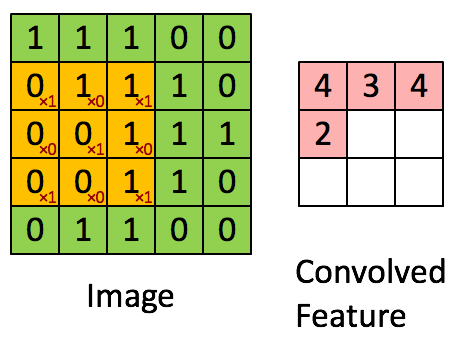
\includegraphics[width=3in]{figures/3_1_参数共享1}
	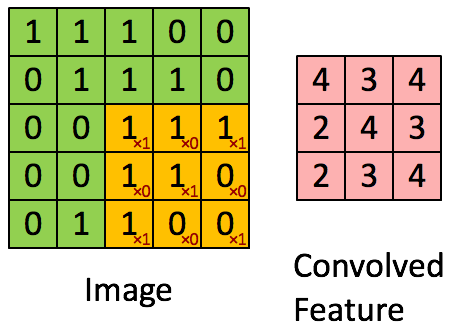
\includegraphics[width=3in]{figures/3_1_参数共享2}
	\caption{卷积核的参数共享} \label{fig:3_1_卷积核的参数共享}
\end{figure}

需要说明的是,一个二维的卷积核只能提取某种特定的特征,而图像中含有多种特征,显然只提取一种特征是非常不充分的。因此卷积层的输入输出一般是多个特征图堆叠起来的3维特征卷(feature volume),此时对应每个输出特征图的卷积核是3维的,或者认为是多个2维的卷积核,每个作用于输入特征卷中的一个特征图,则这些2维的卷积核之间是不共享参数的,如图所示\ref{fig:3_1_三维卷积核}。

\begin{figure}[htb] %三维卷积核
	\centering
	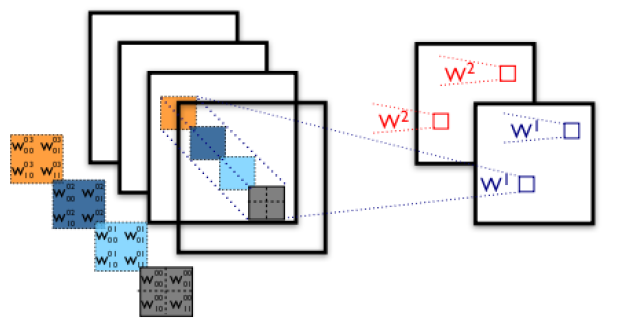
\includegraphics[width=4in]{figures/3_1_三维卷积核}
	\caption{三维卷积核} \label{fig:3_1_三维卷积核}
\end{figure}

%如图\ref{fig:3_1_卷积核的参数共享},输入图像的尺寸是5*5,使用大小为3*3的卷积核来提取图像中的特征,仅需要9个参数。而如果不共享卷积核的参数,则输出的特征图上的每个元素都需要9个参数,输出共有9个元素,故该卷积层需要9*9=81个参数。实际中的图像尺寸远大于9*9,但无论图像多大,卷积核都可以使用3*3的尺寸,则参数共享减少的网络参数数量会更为显著。

我们使用一个具体的例子来定量地分析一下稀疏连接和参数共享在减少网络模型参数数量方面的作用。对于一张尺寸为1000 * 1000的灰度图像,假设输出10个尺寸为500 * 500的特征图,当使用全连接时,该层网络参数共有1000 * 1000 * 500 * 500 * 10 = 2.5e12,如果每个参数占4字节,那么仅保存这些参数就需要9313G的空间,显然这么多的参数是无法训练的。而如果使用尺寸为3*3的卷积核,仅使用稀疏连接时,该层所需参数数量为500 * 500 * 3 * 3 * 10 = 2.25e6,相比2.5e12减小了6个数量级。再加入参数共享,则只需要3 * 3 * 10 = 90个参数。可见,稀疏连接和参数共享在减少网络模型参数数量上的作用是十分惊人的。

(3)等变表示

参数共享使得卷积层具有对平移等变(equivariance)的性质。
函数的等变性指的是函数的输入与输出以相同的方式发生改变,而卷积对平移等变也就是说,对于一张特征图,先对其进行卷积,然后对卷积结果进行平移,与先进行平移再应用卷积的效果是一样的。这也就说明了参数共享能使卷积操作对于整个特征图中的各个位置发挥相同的作用,因而一个特定的卷积核能用于提取散落在特征图中各处的相同特征。卷积对于缩放或旋转等变换并不具有等变性,但通过一些其他机制可以使其具有等变性。
比如,将旋转角度离散化,用多个卷积核各对应一个角度,则当输入旋转某个角度时,总会有一个过滤器被激活,则再使用一个最大池化单元,即可获得对旋转变换的不变性。

%------------------------------------------------------------------------------------
\subsection{卷积神经网络结构}
% ref: 吴正文,ch2.2,p18; 何鹏举,ch2.3,p19; 陈拓,ch3.1.3,p36.
卷积神经网络将传统神经网络的全连接层改为了卷积层,因此其基本网络结构一般包含输入层、卷积层、下采样层和输出层几个部分,有些网络仍然包含全连接层,如图\ref{fig:3_1_卷积神经网络结构}所示。

\begin{figure}[htb] %卷积神经网络结构
	\centering
	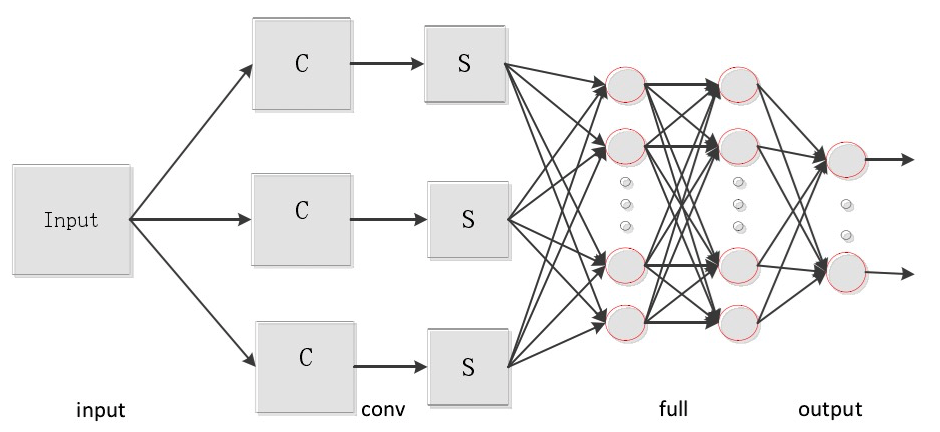
\includegraphics[width=4in]{figures/3_1_卷积神经网络结构}
	\caption{卷积神经网络结构} \label{fig:3_1_卷积神经网络结构}
\end{figure}

输入层:输入层的输入一般为经过某些预处理后的图像,预处理包括灰度化、像素值归一化、裁剪和调整为特定尺寸等。如果把处理后的图像也视为特征图的话,则对于灰度图,输入层为单个特征图,对于彩色图像,输入层为多个特征图,每个对应图像的一个通道。

卷积层:卷积层是卷积神经网络的核心组成部分,其作用是提取图像中的特征,因此也被称为特征提取层。通常卷积层中会使用多个卷积核以提取不同类型的特征,基于每个卷积核可以得到一个特征图(或叫特征平面),故卷积层的输入和输出都是多个特征图堆叠形成的特征卷。卷积层的每个神经元从前一层的局部感受野中提取某种特征,接近输入层的卷积层提取的特征较为低级,在经过多个卷积层之后,特征会逐渐变得更高级、更抽象,同时也会包含更大范围的信息。在对输入的特征图进行卷积运算后,还要像传统神经网络一样加入偏置项(bias),并经过某种类型的非线性激活函数以获得非线性的拟合能力:
%
\begin{equation}
y_l = f(W*y_{l-1}+b)
\end{equation}
$f(\cdot)$表示激活函数。激活函数通常具有非线性、可微性、单调性的性质,常见的激活函数有sigmoid, tanh, 整流线性单元(ReLU)等。sigmoid能把实数范围内的输入压缩到0到1之间输出,但它有一个严重的缺点,当输入非常大或非常小时,函数会饱和,梯度趋向于0,无法实现有效的梯度下降。tanh是sigmoid的变形,tanh(x) = 2sigmoid(2x) - 1,它通常比sigmoid的表现更好,因为其均值为零。整流线性单元不存在饱和的问题,当其处于激活状态时,一阶导数处处为1,因此它的梯度方向效率较高。但它的问题是一旦取值为零,则它的梯度永远为零,也就无法再次激活了,可以认为这个神经元”死亡“了。当设置的学习率较大时,网络中会有大量的神经元死亡。为了解决这个问题,出现了一些ReLU的变种,比如渗透整流线性单元(leaky ReLU)\cite{maas2013rectifier},其定义为f(x,a)=max(0,x)+a*min(x,0),a一般取为类似0.01的小值。
% leaky relu的介绍
\begin{figure}[htb] %激活函数
	\centering
	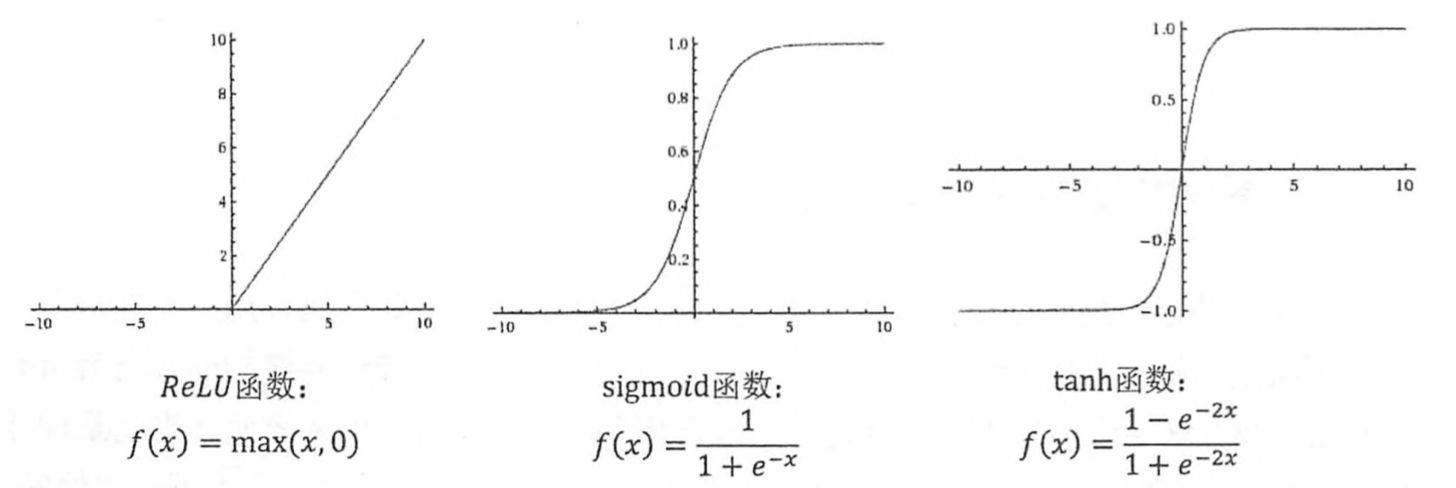
\includegraphics[width=4in]{figures/3_1_激活函数}
	\caption{激活函数} \label{fig:3_1_激活函数}
\end{figure}

每个卷积层的输出尺寸由输入特征图尺寸、卷积核尺寸、步长和边界处的零填充(zero padding)等参数共同决定。设输入、输出特征图分别为边长$x_{i}$和$x_{o}$的正方形,卷积核为边长k的正方形,卷积运算的步长为stride,零填充个数为pad,则输出特征图的尺寸可根据下式来计算:
%
\begin{equation}
x_o = \frac{x_i + 2 \times pad - k}{stride} + 1
\end{equation}


下采样层:下采样层也称为子采样层或池化层,该层的引入是为了在保留有用信息的同时尽量减小数据的维度,本质是一种聚合的操作。下采样的核心是池化函数,它决定了用某一位置所在矩形邻域内的哪一种统计特征作为该位置的输出。池化函数可以表示为:
\begin{equation}
O = (\sum \sum I(i,j)^P \times G(i,j))^{1/P}
\end{equation}
其中,I和O分别表示池化层的输入、输出特征图,G表示高斯核函数,P在$[1, \infty)$内取值。当P=1时,池化被称为平均池化,取各个子区域内元素的均值作为输出;而当$P\rightarrow \infty$时,使用的是最大池化,即输出每个子区域内的最大元素。
如果池化层的输入特征图尺寸为m*n,池化操作水平和竖直方向的步长为w和h,则下采样后输出的特征图尺寸为(m/w)*(n/h)。最常见的采样块尺寸为2*2。
池化操作除了能够降低参数数量外,也能够有效地防止过拟合现象的发生。此外,池化操作还能使卷积层的输出获得局部平移不变性的性质,也就是说,当对该层的输入进行微小的平移时,池化后该层的大多数输出都不会变化。
该性质很重要,因为我们通常只关心某个特征是否出现,而并不关心它的具体位置。

\begin{figure}[htb] %最大池化和平均池化
	\centering
	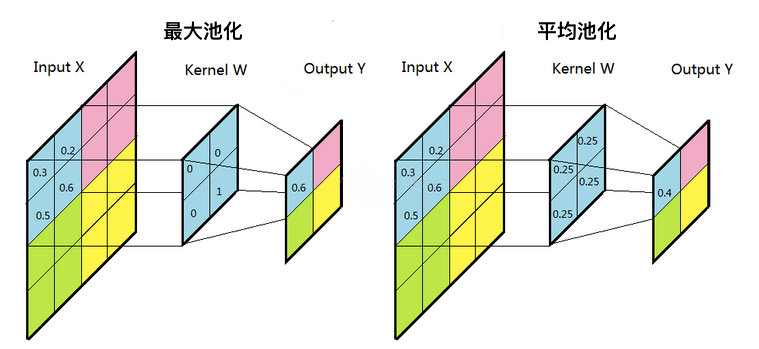
\includegraphics[width=4in]{figures/3_1_最大池化和平均池化}
	\caption{最大池化和平均池化} \label{fig:3_1_最大池化和平均池化}
\end{figure}
%此外,在卷积层中设置卷积的步长和零填充也可以实现下采样的功能。

全连接层:全连接层通常位于最后一个卷积或采样层与输出层之间,用于将二维特征图转变为一维特征向量。全连接层的每个神经元与前一层的每个神经元相连,因此相当于两个矩阵相乘。使用全连接层会给卷积神经网络带来一些限制,因为卷积操作使得卷积层可以接受任意尺寸的输入,而全连接层的神经元个数固定,因此图像尺寸不能随意改变,当输入不同尺寸的图像时,可能需要首先进行缩放或裁剪的处理。

输出层:输出层的设计基于网络的具体应用任务。比如对于图像识别,输出层通常会是一个分类器。常用的分类器包括多项式逻辑回归(Multinomial Logistic Regression)分类器、softmax分类器等,也可以使用一到两层的全连接层作为分类器。
% softmax分类器介绍: 何鹏程, ch2.3.3, p21.

%------------------------------------------------------------------------------------
\subsection{卷积神经网络的训练}
% SGD,反向传播算法;损失函数;正则化。学习率。
\subsubsection{反向传播算法}
% 这块太蛋疼了。。凑活一下吧。。
卷积神经网络的训练与传统人工神经网络的训练类似,主要可以分为有监督、无监督和二者结合等几种方式。本文使用的模型都基于有监督学习,即网络利用带标记的训练样本数据进行学习,训练数据的标记即为监督信号。卷积神经网络的训练本质上是一个优化问题,即定义一个目标函数并将其最小化,该函数也称为代价函数或损失函数。训练常使用基于梯度的方法,主要包括前向传播和反向传播两个阶段。
前向传播即由网络输入经过层层的卷积、池化等操作后求得网络输出的过程,比较简单;反向传播是指由网络的输出值与训练数据的真值之间的误差反向逐层计算各层权重与偏置项的梯度,并根据学习率来更新这些参数使损失函数值逐渐下降至最终收敛。下面简要介绍一下反向传播的计算\cite{bouvrie2006notes}。

% 实在是没有精力看论文推公式了,先抄一下。。
% <Notes on Convolutional Neural Networks>, http://cogprints.org/5869/1/cnn_tutorial.pdf
% http://www.hankcs.com/ml/sgd-cnn.html  (a,z是啥没说明就出现在公式里,看不懂,不用了)
% http://deeplearning.stanford.edu/wiki/index.php/反向传导算法
(1)全连接层的反向传播

令$l$表示当前层,输入层和输出层编号分别为$1$和$L$。定义当前层的输出为$x^l = f(u^l)$,其中$u^l = W^l x^{l-1} + b^l$,$f(\cdot)$表示激活函数。则由下一层传到当前层的残差为:
\begin{equation}\label{eq:3_1_残差_全连接层}
\delta^{l} = ((W^{l+1})^T \delta^{l+1} ) \circ f'(u^l)
\end{equation}
式中$\circ$表示逐元素的乘法。损失函数关于当前层的权重W和偏置b的梯度为:
%% align环境占两行太浪费了,一行挤一挤就好
%\begin{align}
%\frac{\partial E}{\partial W^l} &= x^{l-1}( \delta^l )^T \label{eq:3_1_w梯度_全连接层} \\
%\frac{\partial E}{\partial b^l}  &= \delta^l \label{eq:3_1_b梯度_全连接层}
%\end{align}
\begin{equation}
\frac{\partial E}{\partial W^l} = x^{l-1}( \delta^l )^T, \quad
\frac{\partial E}{\partial b^l}  = \delta^l
\end{equation}


(2)卷积层的反向传播

在卷积层中,每个输出的特征图结合了多个输入特征图的卷积结果。将当前层的输出表示为:
\begin{equation}
x_j^l = f \left( \sum\limits_{i \in M_j} x_i^{l-1} * k_{ij}^l + b_j^l \right)
\end{equation}
式中$M_j$表示输入特征图中的某一个。假设每个卷积层$l$后面都有一个下采样层$l+1$,下采样层中的权重都为$\beta$,则计算残差为:
\begin{equation}
\delta_j^l = \beta_j^{l+1} (f'(u_j^l) \circ up(\delta_j^{l+1})) \label{eq:3_1_残差_卷积层}
\end{equation}
其中$up(\cdot)$表示上采样操作,如果下采样的因子为n,则上采样将每个元素沿水平和竖直方向重复n次。进而可以计算损失关于偏置和卷积核权重的梯度:
%\begin{align}
%\frac{\partial E}{\partial k_{ij}^l} &= \sum\limits_{u,v} (\delta_j^l)_{uv} (p_i^{l-1})_{uv} \label{eq:3_1_w梯度_卷积层} \\
%\frac{\partial E}{\partial b^j}  &= \sum\limits_{u,v} (\delta_j^l)_{uv} \label{eq:3_1_b梯度_卷积层}
%\end{align}
\begin{equation}
\frac{\partial E}{\partial k_{ij}^l} = \sum\limits_{u,v} (\delta_j^l)_{uv} (p_i^{l-1})_{uv} , \quad
\frac{\partial E}{\partial b^j}  = \sum\limits_{u,v} (\delta_j^l)_{uv}
\end{equation}
$(p_i^{l-1})_{uv}$是$x_i^{l-1}$中与卷积核$k_{ij}^l$逐元素相乘的小块。使用MATLAB语句的表示更直观:
\begin{equation}
\frac{\partial E}{\partial k_{ij}^l} = rot180(conv2(x_i^{l-1}, rot180(\delta_j^l), 'valid'))
\end{equation}
'valid'表示卷积的填充方式,旋转180度是为了使用卷积函数来进行互相关操作。

(2)下采样层的反向传播

下采样层的输出表示为:
\begin{equation}
x_j^l = f \left( \beta_j^l down(x_j^{l-1}) + b_j^l \right)
\end{equation}
$down(\cdot)$表示下采样函数。则残差可使用下面的语句求取:
\begin{equation}
\delta_j^l = f'(u_j^l) \circ conv2(\delta_j^{l+1}, rot180(k_j^{l+1}, 'full'))
\end{equation}
定义$d_j^l = down(x_j^{l-1})$,则损失函数关于$b$和$\beta$的梯度分别为:
%\begin{align}
%\frac{\partial E}{\partial b^j}  &= \sum\limits_{u,v} (\delta_j^l)_{uv} \\
%\frac{\partial E}{\partial \beta^j} &= \sum\limits_{u,v} (\delta_j^l \circ d_j^l)_{uv}
%\end{align}
\begin{equation}
\frac{\partial E}{\partial b^j}  = \sum\limits_{u,v} (\delta_j^l)_{uv} , \quad
\frac{\partial E}{\partial \beta^j} = \sum\limits_{u,v} (\delta_j^l \circ d_j^l)_{uv}
\end{equation}

\subsubsection{随机梯度下降}
% SGD, DL book, ch5.10, p160.
% http://www.hankcs.com/ml/sgd-cnn.html
传统梯度下降使用的损失函数通常是对每个输入样本的代价的累积。对于使用n个样本的模型来说,计算每一个梯度的运算代价为O(n)。而深度神经网络的训练需要大量的样本数据,训练集规模可能为上亿的量级,而且模型中的参数也非常多,因此这种计算梯度的策略运算量巨大,非常耗时;另外由于计算机的内存和显存有限,一次性载入大量的训练数据也是不现实的。在这种背景下,随机梯度下降(stochastic gradient descent,SGD)算法应运而生。随机梯度下降的核心思想是,把梯度作为期望来对待,即使用一小部分的样本数据来做一个近似估计。对于训练的每一次迭代,仅从整个训练数据集中抽取很小的一批(minibatch)样本数据用于训练。这个小批量数据的个数m一般取值为1到几百,不论整个训练集的规模增长到多大,m通常都是不变的。算法\ref{alg:sgd}给出了随机梯度下降的具体步骤。
% DL book,ch8.3.1,p279.
\begin{algorithm}[htb]
	\caption{随机梯度下降在第$k$个训练迭代的更新}
	\label{alg:sgd}
	\begin{algorithmic}
		\REQUIRE 学习率 $\epsilon_k$
		\REQUIRE 初始参数$\theta$
		\WHILE{终止训练条件未满足}
		\STATE 从训练数据集中取出$m$个样本$\{ x^{(1)},\dots, x^{(m)}\}$ ,其中$x^{(i)}$对应目标为$y^{(i)}$。
		\STATE 计算梯度的估计值: $\hat{g} \leftarrow + 
		\frac{1}{m} \nabla_{\theta} \sum_i E(f(x^{(i)};\theta),y^{(i)})$
		\STATE 更新参数:$\theta \leftarrow \theta - \epsilon \hat{g}$
		\ENDWHILE
	\end{algorithmic}
\end{algorithm}

学习率是随机梯度下降中的一个很重要的参数。随机梯度下降使用的学习率比普通梯度下降的学习率要小很多,因为其梯度变动比较剧烈,方差较大。在实践中一般要随着迭代次数的增加而逐渐降低学习率,比如可以使用线性衰减的学习率,或者每隔一段时间将学习率减半。更好的方法是预留一部分数据用于每次迭代完成后计算目标函数的输出值,当相邻两次迭代输出的变化小于某个阈值时才减小学习率。一般获取每个批之前要将数据随即打乱,否则得到的梯度可能偏离正确的方向,导致收敛性差。

另外还有很多针对梯度下降的优化算法,如动量法、Adagrad、RMSprop、自适应矩估计(Adam)等,在此不再详细介绍。

\subsubsection{正则化}
% DLbook,ch5.2.2,p132; ch7,p225(L1, L2).
一般我们在训练集之外会使用一个测试集来检验模型的泛化能力,而模型经常会出现欠拟合和过拟合的问题。欠拟合指模型在训练集上不能获得理想的效果,而过拟合指模型在训练集上表现良好,但在测试集上表现很差,训练误差和测试误差之间存在较大的差距。通过调整模型的容量,也就是模型可以选择的函数的数目,可以控制模型对于这两种问题的倾向。根据统计学习理论,随着模型容量变大,训练与泛化误差之差的上界会逐渐增大,因此通过限制模型容量可以改善过拟合现象。

\begin{figure}[htb] %欠拟合和过拟合
	\centering
	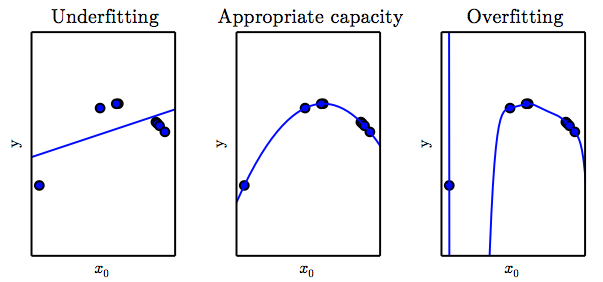
\includegraphics[width=3.5in]{figures/3_1_欠拟合和过拟合}
	\caption{欠拟合和过拟合现象} \label{fig:3_1_欠拟合和过拟合}
\end{figure}

正则化就是用来降低泛化误差、改善过拟合现象的策略。最常见的操作是,在目标函数中加入参数范数的惩罚,从而限制模型参数的增长。对于神经网络中的参数,一般只对权重参数W做惩罚,而不考虑偏置参数b。常用的参数范数惩罚包括L2正则化和L1正则化,分别在目标函数中加入权重的2-范数和1-范数作为惩罚。


%------------------------------------------------------------------------------------
\section{YOLO网络结构}

\section{网络训练}

\section{实验结果}

\section{本章小结}






